\documentclass[11pt, oneside]{article}
\usepackage[margin=.9in]{geometry}
\usepackage{pgfplots}
\pgfplotsset{compat=default}
\newcommand{\cuckoo}{{\rm cuckoo}}
\newcommand{\hash}{{\rm siphash}}
\usepackage{hyperref}
\title{Cuckoo Cycle: \protect\\ a memory-hard proof-of-work system}
\author{John Tromp}
\begin{document}
\maketitle

\begin{abstract}
We introduce the first trivially verifiable, scalable and tmto\footnote{time-memory trade-off}-hard proof-of-work system.
\end{abstract}

\section{Introduction}
A ``proof of work'' (PoW) system allows a verifier to check with
negligible effort that a prover has expended a large amount of computational effort.
Originally introduced as a spam fighting measure, 
where the effort is the price paid by an email sender for demanding the recipient's attention,
they now form one of the cornerstones of crypto-currencies.

Bitcoin\cite{nakamoto2009bitcoin} uses hashcash\cite{back2002} as proof-of-work for
new blocks of transactions, which requires finding a nonce value such that
twofold application of the cryptographic hash function SHA256
to this nonce (and the rest of the block header) results in a number with many
leading 0s.  The bitcoin protocol dynamically adjust this ``difficulty'' number
so as to maintain a 10-minute average block interval. Starting out at 32 leading zeroes in 2009,
the number has steadily climbed and is currently at 63, representing
an incredible $2^{63}/10$ double-hashes per minute. This exponential growth of hashing power
is enabled by the highly-parallellizable nature of the hashcash proof-of-work.
which saw desktop cpus out-performed by graphics-cards (GPUs),
these in turn by field-programmable gate arrays (FPGAs),
and finally by custom designed chips (ASICs).

Downsides of this development include high investment costs, rapid obsolesence,
centralization of mining power, and large power consumption.
This has led people to look for alternative proof-of-work systems that resist parallelizability
and require a nontrivial amount of memory, aiming to keep commodity hardware competitive.

Litecoin replaces the SHA256 hash function in hashcash by a single round version of the
{\em scrypt} key derivation function. Its memory requirement of 128KB is a compromise
between computation-hardness for the prover and verification efficiency for the verifier.
Although designed to be GPU-resistant, GPUs are now at least an order of magnitude faster
than CPUs for Litecoin mining, and ASICs have appeared on the market in early 2014.

Primecoin~\cite{king2013} is an interesting design based on finding long Cunningham chains
of prime numbers, using a two-step process of filtering candidates by {\em sieving}, and applying
pseudo-primality tests to remaining candidates. The most efficient implementations are still CPU based.
Downsides to this proof-of-work are its complexity and the scope for algorithmic improvements
that may be kept private. Its memory requirements, while larger than Litecoin's, are still modest.

Momentum~\cite{larimer2013} proposes finding birthday collisions of hash outputs as proof-of-work,
the simplest way to combine scalable memory usage with trivial verifiability.
Its memory requirements are not very strict though. as Bloom filters or rainbow tables
can identify collisions, and parallellizes well.

Adam Back~\cite{back2014} has a good overview of proof-of-work papers past and present.

\section{Memory latency; the great equalizer}
While cpu-speed and memory bandwidth are highly variable across time and architectures,
main memory latencies have remained relatively stable.
This suggests making the proof-of-work system latency-bound to level the mining playing field.
Ideally, it should have the following properties:
\begin{description}
\item[verify-trivial] A proof can be checked in microseconds rather than milliseconds.
\item[scalable] The amount of memory needed is a parameter that can scale arbitrarily.
\item[linear] Amount of computational steps and memory accesses are linear in the amount of memory.
\item[tmto-hard] Using only half as much memory should incur several orders of magnitude slowdown.
\item[random-access] RAM is accessed randomly, making bandwidth and caches irrelevant.
\item[parallel-hard] No speedup is possible for parallel implementations.
\item[simple] The algorithm should be sufficiently simple that one can be convinced of its optimality.
\end{description}
Combined, these properties ensure that a proof-of-work system is entirely
constrained by main memory latency\footnote{The memory requirement should
exceed that of the largest available
single-chip memory to enforce off-chip latencies. It should also be a
significant fraction of the typical memory of a botnet computer, as sending the
machine into swap-hell is likely to alert its owner.} and scales appropriately
for any application.

We introduce the very first proof-of-work system that is both verify-trivial
and tmto-hard. Furthermore, it satisfies all other properties,
except for parallel-hardness (see the later section on parallelizability).
Amazingly, it amounts to little more than enumerating nonces and storing them
in a hashtable. While all hashtables break down when trying to store more items than
it was designed to handle, in one hashtable design in particular this breakdown
is of a special nature that can be turned into a concise and easily verified proof.
Enter the cuckoo hashtable.

\section{Cuckoo hashing}
Introduced by Rasmus Pagh and Flemming Friche Rodler\cite{Pagh04cuckoohashing},
a cuckoo hashtable consists of two same-sized
tables each with its own hash function mapping a key to a table location,
providing two possible locations for each key.
% (and constant lookup time).
Upon insertion of a new key, if both locations are already occupied by keys,
then one is kicked out and inserted in its alternate location, possibly
displacing yet another key, repeating the process until either a vacant
location is found, or some maximum number of iterations is reached.
The latter can only happen once cycles have formed in the {\em Cuckoo graph}.
This is a bipartite graph with a node for each location and an
edge for every key, connecting the two locations it can reside at.
This naturally suggests a proof-of-work problem, which we now formally define.

\section{The proof-of-work function}
Fix an (even) number of nodes $8 \leq N < 2^{32}$, a number of edges $N/4 < E \leq N$,
and an (even) cycle length $4 \leq L < 256$.
Function $\cuckoo$ maps any 128-bit key $k$ (the header digest) to a bipartite graph
$G = (V_0 \cup V_1, E)$, where $V_0$ is the set of integers modulo $N_0=N/2+1$,
$V_1$ is the set of integers modulo $N_1=N/2-1$, and $E$ has an edge between
$\hash(k,n) \bmod N_0$ in $V_0$ and $\hash(k,n) \bmod N_1$ in $V_1$ for every
nonce $0 \leq n < E$. A proof for $G$ is a subset of $L$ nonces whose
corresponding edges form an $L$-cycle in $G$.

\section{Solving the proof-of-work problem}
We enumerate the $E$ nonces, but instead of storing the nonce itself as a key
in the Cuckoo hashtable, we store the alternate key location at the key location,
and forget about the nonce.
We thus maintain the {\em directed} cuckoo graph, in which the edge for a key
is directed from the location where it resides to its alternate location.
Moving a key to its alternate location thus corresponds to reversing its edge.
The outdegree of every node in this graph is either 0 or 1.
When there are no cycles yet, the graph is a {\em forest}, a disjoint union of trees.
In each tree, all edges are directed, directly, or indirectly, to its {\em root},
the only node in the tree with outdegree 0.
Initially there are just $N$ singleton trees consisting of individual nodes which are all roots.
Addition of a new key causes a cycle if and only if its two endpoints are nodes in the same tree,
which we can test by following the path from each endpoint to its root.
In case of different roots, we reverse all edges on the shorter of the two paths,
and finally create the edge for the new key itself, thereby joining the two trees into one.
The left diagram below shows the directed cuckoo graph for header `header' on $N=9+7$ nodes after adding edges
$(3,16),(5,15),(6,16),(7,16),(5,10),(6,13),(6,12),(9,14)$ and $(4,14)$ (nodes with no incident edges are omitted for clarity).
In order to add the 10th edge $(7,10)$, we follow the paths $7 \rightarrow 16 \rightarrow 3$ and $10 \rightarrow 5$
to find different roots $3$ and $5$. Since the latter path is shorter, we reverse it to $5 \rightarrow 10$ so we can
add the new edge as $(10 \rightarrow 7)$, resulting in the right diagram.
\begin{center}
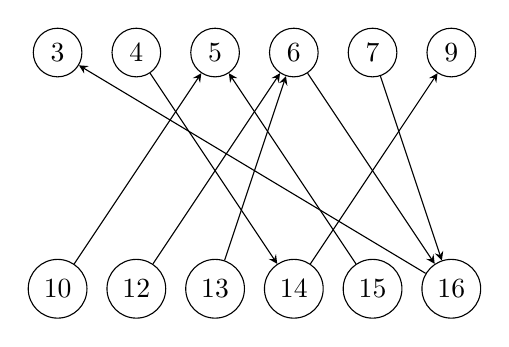
\begin{tikzpicture}[>=stealth]
\node  (3) at (1, 2) [shape=circle,draw] {3};
\node  (4) at (2, 2) [shape=circle,draw] {4};
\node  (5) at (3, 2) [shape=circle,draw] {5};
\node  (6) at (4, 2) [shape=circle,draw] {6};
\node  (7) at (5, 2) [shape=circle,draw] {7};
\node  (9) at (6, 2) [shape=circle,draw] {9};
\node (10) at (1,-1) [shape=circle,draw] {10};
\node (12) at (2,-1) [shape=circle,draw] {12};
\node (13) at (3,-1) [shape=circle,draw] {13};
\node (14) at (4,-1) [shape=circle,draw] {14};
\node (15) at (5,-1) [shape=circle,draw] {15};
\node (16) at (6,-1) [shape=circle,draw] {16};
\draw [->] (16) -- (3);
\draw [->] (15) -- (5);
\draw [->]  (6) -- (16);
\draw [->]  (7) -- (16);
\draw [->] (10) -- (5);
\draw [->] (13) -- (6);
\draw [->] (12) -- (6);
\draw [->] (14) -- (9);
\draw [->]  (4) -- (14);
\end{tikzpicture}\hspace{3cm}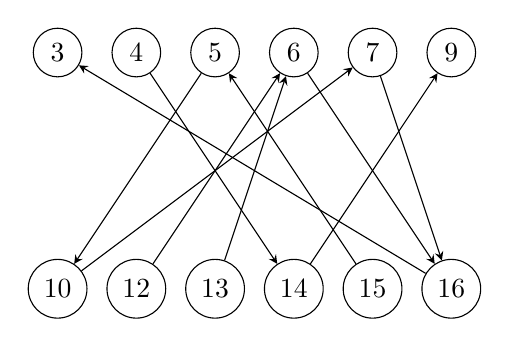
\begin{tikzpicture}[>=stealth]
\node  (3) at (1, 2) [shape=circle,draw] {3};
\node  (4) at (2, 2) [shape=circle,draw] {4};
\node  (5) at (3, 2) [shape=circle,draw] {5};
\node  (6) at (4, 2) [shape=circle,draw] {6};
\node  (7) at (5, 2) [shape=circle,draw] {7};
\node  (9) at (6, 2) [shape=circle,draw] {9};
\node (10) at (1,-1) [shape=circle,draw] {10};
\node (12) at (2,-1) [shape=circle,draw] {12};
\node (13) at (3,-1) [shape=circle,draw] {13};
\node (14) at (4,-1) [shape=circle,draw] {14};
\node (15) at (5,-1) [shape=circle,draw] {15};
\node (16) at (6,-1) [shape=circle,draw] {16};
\draw [->] (16) -- (3);
\draw [->] (15) -- (5);
\draw [->]  (6) -- (16);
\draw [->]  (7) -- (16);
\draw [->]  (5) -- (10);
\draw [->] (13) -- (6);
\draw [->] (12) -- (6);
\draw [->] (14) -- (9);
\draw [->]  (4) -- (14);
\draw [->] (10) -- (7);
\end{tikzpicture}
\end{center}
When adding the 11th edge $(3,15)$, we find the singleton path $3$ and the path
$15 \rightarrow 5 \rightarrow 10 \rightarrow 7 \rightarrow 16 \rightarrow 3$ with equal roots.
In this case, we can compute the length of the resulting cycle as
1 plus the sum of the path-lengths to the node where the two paths first join.
In the diagram, the paths first join at the root, and the cycle length is computed as $1+0+5=6$.
If the cycle length equals $L$, then we solved the problem, and recover the proof
by enumerating nonces once more and checking which ones formed the cycle.
If not, then we keep the graph acyclic by ignoring the edge.
There is some probability of overlooking other $L$-cycles
through that edge, but in the important case of having few cycles
in the cuckoo graph to begin with, it hardly affects the rate of solution finding.

\section{Implementation and performance}
The C-program listed in the Appendix is also available online at
\url{https://github.com/tromp/cuckoo} together with a Makefile,
proof verifier and the latest version of this paper. `make test' tests everything.
`make example' reproduces the example shown above.
The main program uses 31 bits per node to represent the
directed cuckoo graph, reserving the most significant bit
for marking edges on a cycle, to simplify recovery of the proof nonces.
The left plot below shows both the total runtime in seconds and the runtime of just
the hash computation, as a function of (log)size. The latter is purely
linear, while the former is superlinear due to increasing memory latency
as the nodes no longer fit in cache. The right plot show this more clearly
as the percentage of hashing to total runtime, ending up around 5\%.

\begin{center}
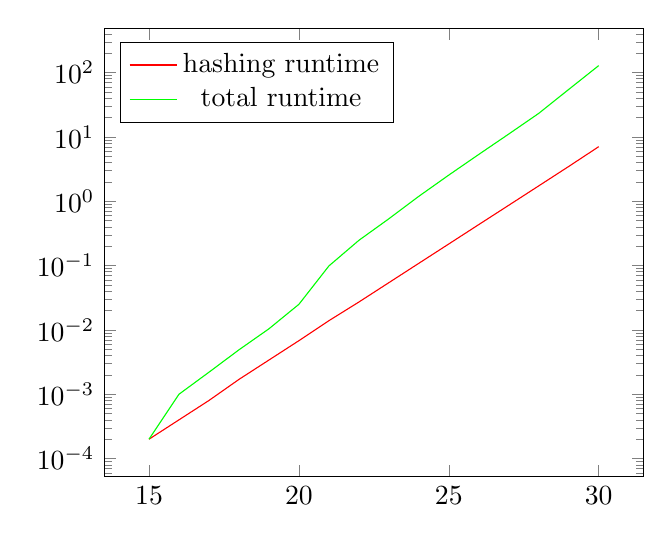
\begin{tikzpicture}
\begin{axis}[ymode=log, legend pos=north west]
\addplot[color=red] coordinates {
% (10,0.0000) (11,0.0000) (12,0.0000) (13,0.0001) (14,0.0001)
(15,0.0002) (16,0.0004) (17,0.0008) (18,0.0017) (19,0.0034)
(20,0.0068) (21,0.0139) (22,0.0271) (23,0.0542) (24,0.1084)
(25,0.2166) (26,0.4336) (27,0.8658) (28,1.7322) (29,3.4719)
(30,7.0389) };
\addlegendentry{hashing runtime}
\addplot[color=green] coordinates {
% (10,0.0000) (11,0.0000) (12,0.0001) (13,0.0001) (14,0.0003)
(15,0.0002) (16,0.0010) (17,0.0022) (18,0.0049) (19,0.0104)
(20,0.0250) (21,0.0986) (22,0.2465) (23,0.5332) (24,1.1922)
(25,2.5505) (26,5.3394) (27,11.0793) (28,23.1984) (29,54.6811)
(30,128.1682) };
\addlegendentry{total runtime}
\end{axis}
\end{tikzpicture}
\hspace{1cm}
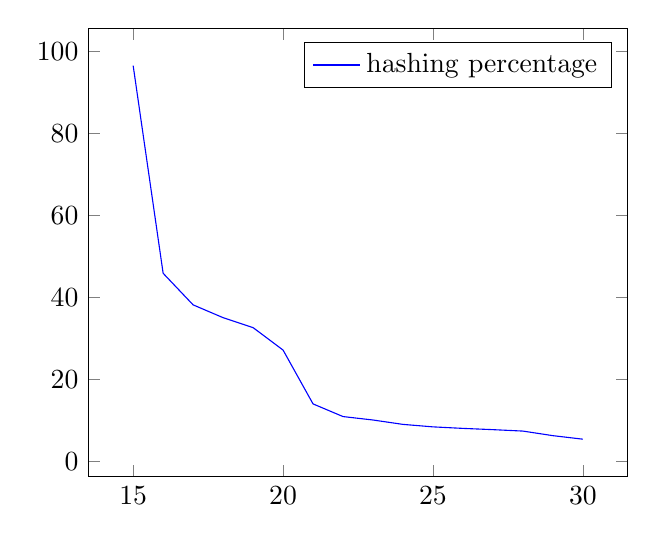
\begin{tikzpicture}
\begin{axis}[legend pos=north east]
\addplot[color=blue] coordinates {
% (10,38.8889) (11,33.3333) (12,45.1613) (13,39.8496) (14,44.6154)
(15,96.5217) (16,45.9119) (17,38.2180) (18,35.0988) (19,32.6724)
(20,27.2076) (21,14.0874) (22,11.0014) (23,10.1635) (24,9.0964)
(25,8.4921) (26,8.1215) (27,7.8144) (28,7.4670) (29,6.3494)
(30,5.4919) };
\addlegendentry{hashing percentage}
\end{axis}
\end{tikzpicture}
\end{center}

% A simultaneous multithreading (SMT) implementation should be able to
% completely hide the hash computations inside memory access latencies for the bigger sizes.
On a 3.2GHz Intel Core i5, size $2^{20}$ takes 4MB and 0.025s, size
$2^{25}$ takes 128MB and 2.5s, and size $2^{30}$ takes 4GB and 128s, or roughly half a minute per GB.
The left plot below shows the probability of finding a 42-cycle as a function
of the percentage edges/nodes (relative easiness), while the right plot shows the average number of
memory reads and writes per edge as a function of the percentage
nonce/easiness (progress through main loop). Both were determined from 10000 runs at size $2^{20}$;
results at size $2^{25}$ look almost identical.
In total the program averages 3.3 reads and 1.1 writes per edge.

\begin{center}
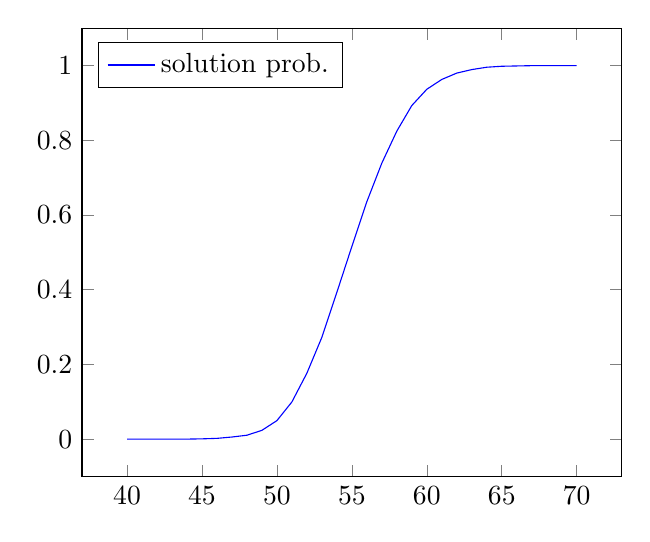
\begin{tikzpicture}
\begin{axis}[legend pos=north west]
\addplot[color=blue] coordinates {
% (1,0) (2,0) (3,0) (4,0) (5,0) (6,0) (7,0) (8,0) (9,0) (10,0)
% (11,0) (12,0) (13,0) (14,0) (15,0) (16,0) (17,0) (18,0) (19,0) (20,0)
% (21,0) (22,0) (23,0) (24,0) (25,0) (26,0) (27,0) (28,0) (29,0) (30,0)
% (31,0) (32,0) (33,0) (34,0) (35,0) (36,0) (37,0) (38,0) (39,0)
(40,0) (41,0) (42,0) (43,0.0001) (44,0.0002) (45,0.0009)
(46,0.0022) (47,0.0058) (48,0.0106) (49,0.0237) (50,0.0497)
(51,0.0997) (52,0.1767) (53,0.2728) (54,0.3931) (55,0.5158)
(56,0.6357) (57,0.739) (58,0.8246) (59,0.8931) (60,0.9366)
(61,0.9629) (62,0.9799) (63,0.9893) (64,0.9956) (65,0.9982)
(66,0.999) (67,0.9998) (68,1) (69,1) (70,1)
% (71,1) (72,1) (73,1) (74,1) (75,1) (76,1) (77,1) (78,1) (79,1) (80,1)
% (81,1) (82,1) (83,1) (84,1) (85,1) (86,1) (87,1) (88,1) (89,1) (90,1)
% (91,1) (92,1) (93,1) (94,1) (95,1) (96,1) (97,1) (98,1) (99,1) (100,1)
};
\addlegendentry{solution prob.}
\end{axis}
\end{tikzpicture}
\hspace{1cm}
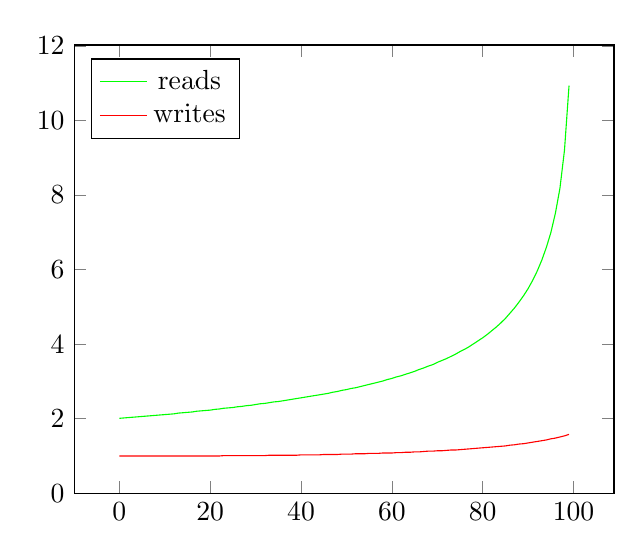
\begin{tikzpicture}
\begin{axis}[ymin=0, legend pos=north west]
\addplot[color=green] coordinates {
(0,2.01) (1,2.02) (2,2.03) (3,2.04) (4,2.05) (5,2.06) (6,2.07) (7,2.08) (8,2.09) (9,2.10) (10,2.11) (11,2.12) (12,2.13) (13,2.15) (14,2.16) (15,2.17) (16,2.18) (17,2.20) (18,2.21) (19,2.22) (20,2.23) (21,2.25) (22,2.26) (23,2.28) (24,2.29) (25,2.30) (26,2.32) (27,2.33) (28,2.35) (29,2.36) (30,2.38) (31,2.40) (32,2.41) (33,2.43) (34,2.45) (35,2.46) (36,2.48) (37,2.50) (38,2.52) (39,2.54) (40,2.56) (41,2.58) (42,2.60) (43,2.62) (44,2.64) (45,2.66) (46,2.68) (47,2.71) (48,2.73) (49,2.76) (50,2.78) (51,2.81) (52,2.83) (53,2.86) (54,2.89) (55,2.92) (56,2.95) (57,2.98) (58,3.01) (59,3.05) (60,3.08) (61,3.12) (62,3.15) (63,3.19) (64,3.23) (65,3.27) (66,3.32) (67,3.36) (68,3.41) (69,3.45) (70,3.51) (71,3.56) (72,3.61) (73,3.67) (74,3.73) (75,3.80) (76,3.86) (77,3.93) (78,4.01) (79,4.09) (80,4.17) (81,4.26) (82,4.36) (83,4.46) (84,4.57) (85,4.69) (86,4.83) (87,4.97) (88,5.13) (89,5.30) (90,5.49) (91,5.71) (92,5.96) (93,6.25) (94,6.59) (95,6.99) (96,7.51) (97,8.18) (98,9.20) (99,10.93) };
\addlegendentry{reads}
\addplot[color=red] coordinates {
(0,1.00) (1,1.00) (2,1.00) (3,1.00) (4,1.00) (5,1.00) (6,1.00) (7,1.00) (8,1.00) (9,1.00) (10,1.00) (11,1.00) (12,1.00) (13,1.00) (14,1.00) (15,1.00) (16,1.00) (17,1.00) (18,1.00) (19,1.00) (20,1.00) (21,1.00) (22,1.00) (23,1.01) (24,1.01) (25,1.01) (26,1.01) (27,1.01) (28,1.01) (29,1.01) (30,1.01) (31,1.01) (32,1.01) (33,1.02) (34,1.02) (35,1.02) (36,1.02) (37,1.02) (38,1.02) (39,1.02) (40,1.03) (41,1.03) (42,1.03) (43,1.03) (44,1.03) (45,1.04) (46,1.04) (47,1.04) (48,1.04) (49,1.05) (50,1.05) (51,1.05) (52,1.06) (53,1.06) (54,1.06) (55,1.07) (56,1.07) (57,1.07) (58,1.08) (59,1.08) (60,1.08) (61,1.09) (62,1.09) (63,1.10) (64,1.10) (65,1.11) (66,1.11) (67,1.12) (68,1.13) (69,1.13) (70,1.14) (71,1.14) (72,1.15) (73,1.16) (74,1.16) (75,1.17) (76,1.18) (77,1.19) (78,1.20) (79,1.21) (80,1.22) (81,1.23) (82,1.24) (83,1.25) (84,1.26) (85,1.27) (86,1.29) (87,1.30) (88,1.32) (89,1.33) (90,1.35) (91,1.37) (92,1.39) (93,1.41) (94,1.43) (95,1.46) (96,1.48) (97,1.51) (98,1.54) (99,1.58) };
\addlegendentry{writes}
\end{axis}
\end{tikzpicture}
\end{center}

\section{Difficulty control}
Relative easiness (the ratio $E/N$) determines a base level of difficulty,
which may suffice for applications where difficulty is to remain fixed.
The ratio $E/N=1$ is suitable when a practically guaranteed solution is desired,
For crypto currencies, where difficulty must scale in precisely
controlled manner across a huge range, adjusting easiness is not suitable.
The implementation default $E/N=1/2$ gives a solution probability of roughly $5\%$,
while keeping the number of found cycles down to a handful.
For further control, a diffculty target $0 < T < 2^{64}$ is introduced,
and we impose the additional constraint $\hash(h,\Sigma) < T$
on any $L$-cycle, where $\Sigma$ is the sum of its nonces modulo $E$.
This reduces the success probability by a factor $2^{64}/T$.

\section{Memory-hardness}
I conjecture that this problem doesn't allow for a time-memory trade-off. If
one were to store only a fraction $p$ of $V_0$ and $V_1$, then one would have
to reject a fraction $p^2$ of generated edges, drastically reducing the odds of
finding cycles for $p<1/\sqrt{2}$ (the reduction being exponential in cycle length).
There is one obvious trade-off in the other direction. By doubling the memory
used, nonces can be stored alongside the directed edges, which would save the
effort of recovering them in the current slow manner. The speedup only
applies to solution finding runs though, so a better use of that memory would be to run
another copy in parallel.

\section{Parallelizability}
The implementation allows the number of threads to be set with -DNTHREADS.
For $0\leq t < T$, thread $t$ processes all nonces $t \bmod T$.
Parallelization presents some algorithmic challenges. Paths from an edge's two endpoints
are not well-defined when other edge additions and path reversals are still in progress.
One example of such a path conflict is the addition of edges
$(7,10)$ and $(3,15)$ in the example diagrams. If these were to happen in parallel,
then the path from $15$ will likely end at $5$ because
edge $(10 \rightarrow 5)$ hasn't been reversed yet.
As a result, $(3 \rightarrow 15)$ will be added, not realizing it creates a cyle.
Thus, in a parallel implementation, path following can no longer be assumed to terminate.
Instead of using a cycle detection algorithm such as~\cite{1980-brent-cycles}, our implementation
simply aborts when the path length exceeds MAXPATHLEN.
The left plot below shows the average number of times that either of the two roots
for a nonce occurred a given number of nonces ago, showing that there are potentially
about $10T$ such conflicts.
% Analysing how these conflicts affect performance and the probabillity of finding cycles
% is a topic for further research. 
The right plot shows the speedup achieved by up to 12 threads on an Intel Xeon X5670 at 2.93GHz.
Each datapoint represents 10 runs on $2^{30}$ nodes with headers "0" through "9".
Although the speedup is sublinear at 8.7 for 12 threads, there are still clear gains to be made
by using more threads. Since there were no aborts in the 110 multithreaded runs, path conflicts
do not pose a problem yet. More experiments are needed to determine where memory bottlenecks
and path conflicts make further multithreading ineffective.
% Note that unless one uses at least $P^2$ MEs, memory routing conflicts will frequently arise.
% The possibility of development of custom hardware for improved parallel random access to global
% shared memory need not be a big concern, as this is likely to benefit many other applications as well.

\begin{center}
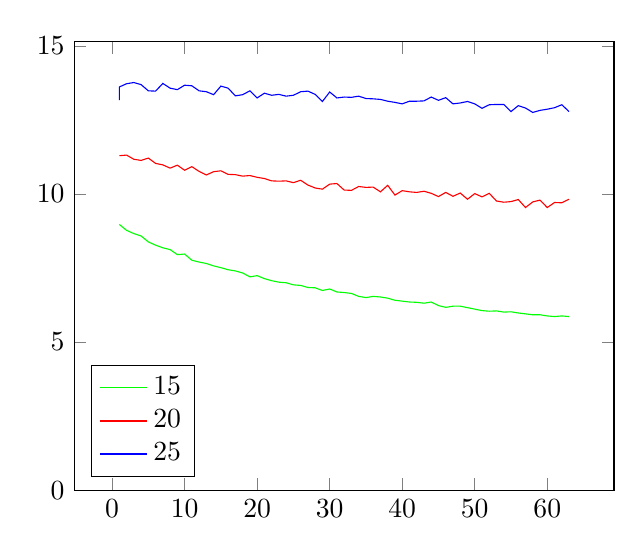
\begin{tikzpicture}
\begin{axis}[ymin=0, legend pos=south west]
\addplot[color=green] coordinates {
(1, 8.97) (2, 8.77) (3, 8.66) (4, 8.58) (5, 8.38) (6, 8.27) (7, 8.18) (8, 8.12) (9, 7.95) (10, 7.97) (11, 7.76) (12, 7.70) (13, 7.65) (14, 7.57) (15, 7.51) (16, 7.44) (17, 7.40) (18, 7.33) (19, 7.20) (20, 7.24) (21, 7.14) (22, 7.07) (23, 7.02) (24, 7.00) (25, 6.93) (26, 6.91) (27, 6.84) (28, 6.83) (29, 6.74) (30, 6.79) (31, 6.69) (32, 6.67) (33, 6.64) (34, 6.54) (35, 6.50) (36, 6.54) (37, 6.52) (38, 6.48) (39, 6.41) (40, 6.38) (41, 6.35) (42, 6.34) (43, 6.31) (44, 6.35) (45, 6.23) (46, 6.17) (47, 6.21) (48, 6.21) (49, 6.16) (50, 6.11) (51, 6.06) (52, 6.04) (53, 6.05) (54, 6.01) (55, 6.02) (56, 5.98) (57, 5.95) (58, 5.92) (59, 5.92) (60, 5.88) (61, 5.86) (62, 5.88) (63, 5.86) };
\addlegendentry{15}
\addplot[color=red] coordinates {
(1,11.29) (2,11.31) (3,11.17) (4,11.13) (5,11.21) (6,11.03) (7,10.98) (8,10.87) (9,10.97) (10,10.80) (11,10.92) (12,10.76) (13,10.64) (14,10.75) (15,10.78) (16,10.66) (17,10.65) (18,10.60) (19,10.62) (20,10.56) (21,10.52) (22,10.44) (23,10.43) (24,10.44) (25,10.38) (26,10.46) (27,10.30) (28,10.20) (29,10.16) (30,10.33) (31,10.35) (32,10.13) (33,10.12) (34,10.25) (35,10.22) (36,10.23) (37,10.07) (38,10.29) (39, 9.96) (40,10.11) (41,10.07) (42,10.05) (43,10.09) (44,10.02) (45, 9.91) (46,10.05) (47, 9.92) (48,10.03) (49, 9.82) (50,10.01) (51, 9.90) (52,10.02) (53, 9.76) (54, 9.72) (55, 9.74) (56, 9.81) (57, 9.54) (58, 9.73) (59, 9.79) (60, 9.54) (61, 9.71) (62, 9.70) (63, 9.82) };
\addlegendentry{20}
\addplot[color=blue] coordinates {
(1,13.17)(1,13.61) (2,13.72) (3,13.76) (4,13.69) (5,13.48) (6,13.47) (7,13.73) (8,13.57) (9,13.52) (10,13.67) (11,13.65) (12,13.48) (13,13.45) (14,13.35) (15,13.64) (16,13.57) (17,13.31) (18,13.35) (19,13.48) (20,13.24) (21,13.40) (22,13.33) (23,13.36) (24,13.30) (25,13.33) (26,13.45) (27,13.47) (28,13.36) (29,13.12) (30,13.44) (31,13.24) (32,13.27) (33,13.26) (34,13.30) (35,13.22) (36,13.21) (37,13.19) (38,13.13) (39,13.09) (40,13.04) (41,13.13) (42,13.13) (43,13.14) (44,13.27) (45,13.16) (46,13.25) (47,13.04) (48,13.07) (49,13.12) (50,13.04) (51,12.89) (52,13.01) (53,13.02) (54,13.02) (55,12.78) (56,12.98) (57,12.90) (58,12.75) (59,12.82) (60,12.86) (61,12.91) (62,13.01) (63,12.78) };
\addlegendentry{25}
\end{axis}
\end{tikzpicture}\hspace{1cm}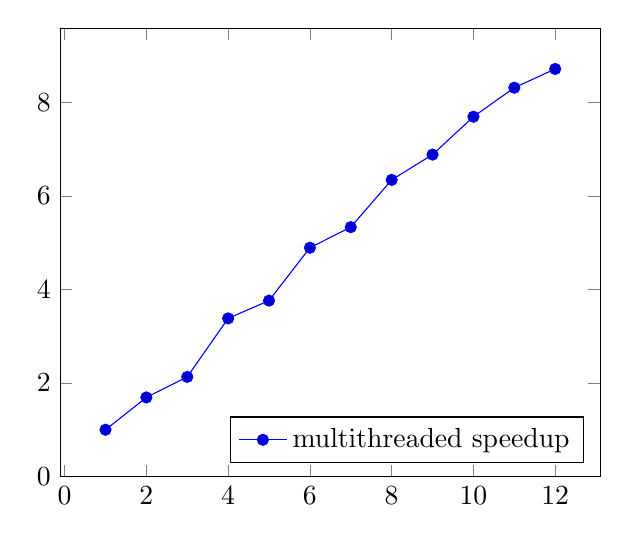
\begin{tikzpicture}
\begin{axis}[ymin=0, legend pos=south east]
\addplot coordinates { (1, 1) (2, 1.69) (3, 2.13) (4, 3.38) (5, 3.76)
(6, 4.89) (7, 5.33) (8, 6.34) (9, 6.88) (10, 7.69) (11, 8.31) (12, 8.71) };
\addlegendentry{multithreaded speedup}
\end{axis}
\end{tikzpicture}
\end{center}

\section{Choice of cycle length}
Extremely small cycle lengths risk the feasability of alternative datastructures that
are more memory-efficient. For example, for $L=2$ the problem reduces to finding a birthday collision
as in the Momentum proof-of-work.
It is conceivable however that the Cuckoo representation is already optimal for $L=4$.
Such small values still harm the TMTO resistance though, as mentioned in the previous paragraph,
and may reduce parallelization resistance.
In order to keep proof size manageable, the cycle length should not be too large either.
We consider 20-64 to be a healthy range, which averages to 42.
The plot below shows the distribution of cycle lengths found for sizes $2^{10},2^{15},2^{20},2^{25}$,
as determined from 100000,100000,10000, and 10000 runs respectively. The tails of the distributions
beyond $L=100$ are not shown. For reference, the longest cycle found was of length 2120.

\begin{center}
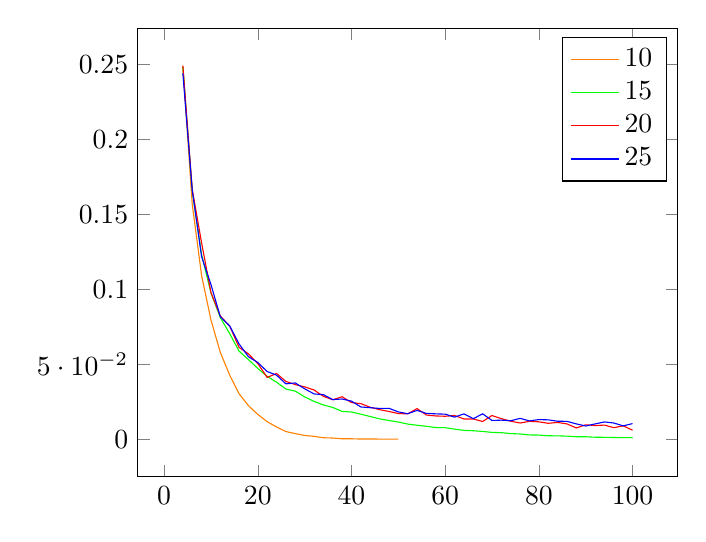
\begin{tikzpicture}
\begin{axis}
\addplot[color=orange] coordinates {
(4,0.24862) (6,0.15673) (8,0.10907) (10,0.07952) (12,0.05783) (14,0.04269) (16,0.0303)
(18,0.02237) (20,0.01653) (22,0.01168) (24,0.00815) (26,0.00511) (28,0.00374) (30,0.00251)
(32,0.00191) (34,0.00098) (36,0.00079) (38,0.00029) (40,0.0003) (42,0.00011) (44,0.00018)
(46,8e-05) (48,2e-05) (50,3e-05) };
\addlegendentry{10}
\addplot[color=green] coordinates {
(4,0.24822) (6,0.16551) (8,0.12317) (10,0.09749) (12,0.08105) (14,0.07036) (16,0.05871) (18,0.05308)
(20,0.04717) (22,0.04189) (24,0.03801) (26,0.03342) (28,0.03205) (30,0.02822) (32,0.02521)
(34,0.02282) (36,0.0212) (38,0.01852) (40,0.01814) (42,0.01668) (44,0.01511) (46,0.01356)
(48,0.01246) (50,0.01145) (52,0.0101) (54,0.0093) (56,0.00861) (58,0.00778) (60,0.00768)
(62,0.00672) (64,0.00589) (66,0.00565) (68,0.00517) (70,0.00455) (72,0.00435) (74,0.00375)
(76,0.00348) (78,0.00286) (80,0.00276) (82,0.0023) (84,0.00224) (86,0.00204) (88,0.00165)
(90,0.00164) (92,0.00134) (94,0.00126) (96,0.00114) (98,0.00103) (100,0.00101) };
\addlegendentry{15}
\addplot[color=red] coordinates {
(4,0.249) (6,0.1666) (8,0.1309) (10,0.0977) (12,0.0821) (14,0.0754) (16,0.0612) (18,0.0569)
(20,0.0504) (22,0.0412) (24,0.0438) (26,0.0385) (28,0.0364) (30,0.0349) (32,0.0328) (34,0.0286)
(36,0.0263) (38,0.0283) (40,0.0244) (42,0.0237) (44,0.0213) (46,0.0197) (48,0.0185) (50,0.0171)
(52,0.0169) (54,0.0204) (56,0.0161) (58,0.0155) (60,0.0153) (62,0.0158) (64,0.0135) (66,0.0135)
(68,0.0118) (70,0.0158) (72,0.0137) (74,0.012) (76,0.0108) (78,0.0119) (80,0.0116) (82,0.0106)
(84,0.0112) (86,0.0102) (88,0.0075) (90,0.0096) (92,0.0091) (94,0.0094) (96,0.0077) (98,0.0089)
(100,0.006) };
\addlegendentry{20}
\addplot[color=blue] coordinates {
(4,0.2439) (6,0.1661) (8,0.1216) (10,0.1031) (12,0.0816) (14,0.0755) (16,0.0635) (18,0.055) (20,0.0511) (22,0.0451) (24,0.0427) (26,0.0369) (28,0.0375) (30,0.0336) (32,0.0302) (34,0.0297) (36,0.0264) (38,0.0268) (40,0.0254) (42,0.0215) (44,0.021) (46,0.0205) (48,0.0206) (50,0.0182) (52,0.017) (54,0.0192) (56,0.0172) (58,0.0169) (60,0.0167) (62,0.0147) (64,0.0169) (66,0.0137) (68,0.0169) (70,0.0125) (72,0.0127) (74,0.0123) (76,0.0139) (78,0.0122) (80,0.0131) (82,0.0129) (84,0.012) (86,0.0119) (88,0.0102) (90,0.0088) (92,0.0102) (94,0.0115) (96,0.0108) (98,0.0089) (100,0.0104) };
\addlegendentry{25}
\end{axis}
\end{tikzpicture}
\end{center}

\section{Scaling memory beyond 16-32 GB}
While the current algorithm can accomodate up to $N=2^{33}-2$ nodes by a simple change
in implementation, a different idea is needed to scale beyond that.
To that end, we propose to use $K$-partite graphs with edges only between partition $k$ and partition $(k+1) \bmod K$,
where $k$ is fed into the hash function along with the header and nonce. With each partition consisting of at most
$2^{31}-1$ nodes, the most significant bit is then available to distinguish edges to the two neighbouring partitions.
The partition sizes should remain relatively prime, e.g. by picking the largest $K$ primes under $2^{31}$.

\section{Conclusion}
Cuckoo Cycle is an elegant proof-of-work design emphasizing memory latency over computation.
This promotes investment in low-power general purpose hardware (RAM) rather than investment
in single purpose hardware coupled with high operational costs, making mining more sustainable.
More research is needed to determine the limits of parallelizability.

\bibliographystyle{IEEEtran}
\bibliography{cuckoo}

\section{Appendix A: cuckoo.c Source Code}
\footnotesize
\begin{verbatim}
// Cuckoo Cycle, a memory-hard proof-of-work
// Copyright (c) 2013-2014 John Tromp

#include "cuckoo.h"
// algorithm parameters
#define MAXPATHLEN 8192

// used to simplify nonce recovery
#define CYCLE 0x80000000
unsigned cuckoo[1+SIZE]; // global; conveniently initialized to zero
pthread_t threads[NTHREADS];
pthread_mutex_t setsol = PTHREAD_MUTEX_INITIALIZER;
unsigned solus[MAXPATHLEN], solnu, solvs[MAXPATHLEN], solnv; 

void *worker(void *tp) {
  int t = (pthread_t *)tp - threads;
  unsigned us[MAXPATHLEN], nu, u, vs[MAXPATHLEN], nv, v; 
  for (unsigned nonce = t; nonce < EASINESS; nonce += NTHREADS) {
    sipedge(nonce, us, vs);
    if ((u = cuckoo[*us]) == *vs || (v = cuckoo[*vs]) == *us)
      continue; // ignore duplicate edges
    for (nu = 0; u; u = cuckoo[u]) {
      assert(nu < MAXPATHLEN-1);
      us[++nu] = u;
    }
    for (nv = 0; v; v = cuckoo[v]) {
      assert(nv < MAXPATHLEN-1);
      vs[++nv] = v;
    }
#ifdef SHOW
    for (int j=1; j<=SIZE; j++)
      if (!cuckoo[j]) printf("%2d:   ",j);
      else            printf("%2d:%02d ",j,cuckoo[j]);
    printf(" %x (%d,%d)\n", nonce,*us,*vs);
#endif
    if (us[nu] == vs[nv]) {
      int min = nu < nv ? nu : nv;
      for (nu -= min, nv -= min; us[nu] != vs[nv]; nu++, nv++) ;
      int len = nu + nv + 1;
      printf("% 4d-cycle found at %d:%d%%\n", len, t, (int)(nonce*100L/EASINESS));
      if (len != PROOFSIZE)
        continue;
      pthread_mutex_lock(&setsol);
      for (solnu = nu, nu = 0; nu <= solnu; nu++)
        solus[nu] = us[nu];
      for (solnv = nv, nv = 0; nv <= solnv; nv++)
        solvs[nv] = vs[nv];
      pthread_mutex_unlock(&setsol);
    } else if (nu < nv) {
      while (nu--)
        cuckoo[us[nu+1]] = us[nu];
      cuckoo[*us] = *vs;
    } else {
      while (nv--)
        cuckoo[vs[nv+1]] = vs[nv];
      cuckoo[*vs] = *us;
    }
  }
  pthread_exit(NULL);
}

int main(int argc, char **argv) {
  // 6 largest sizes 131 928 529 330 729 132 not implemented
  assert(SIZE < (unsigned)CYCLE);
  char *header = argc >= 2 ? argv[1] : "";
  setheader(header);
  printf("Looking for %d-cycle on cuckoo%d%d(\"%s\") with %d edges\n",
               PROOFSIZE, SIZEMULT, SIZESHIFT, header, EASINESS);
  for (int t = 0; t < NTHREADS; t++)
    assert(pthread_create(&threads[t], NULL, worker, (void *)&threads[t]) == 0);
  for (int t = 0; t < NTHREADS; t++)
    assert(pthread_join(threads[t], NULL) == 0);
  if (!solnu)
    return 0;
  while (solnu--)
    cuckoo[solus[solnu]] = CYCLE | solus[solnu+1];
  while (solnv--)
    cuckoo[solvs[solnv+1]] = CYCLE | solvs[solnv];
  cuckoo[*solvs] = CYCLE | *solus;
  unsigned len = 0, u, v;
  for (unsigned nonce = 0; nonce < EASINESS ; nonce++) {
    sipedge(nonce, &u, &v);
    unsigned c;
    if (cuckoo[c=u] == (CYCLE|v) || cuckoo[c=v] == (CYCLE|u)) {
      printf("%2d %08x (%d,%d)\n", len++, nonce, u, v);
      cuckoo[c] &= ~CYCLE;
    }
  }
  return 0;
}
\end{verbatim}

\section{Appendix B: cuckoo.h Header File}
\footnotesize
\begin{verbatim}
// Cuckoo Cycle, a memory-hard proof-of-work
// Copyright (c) 2013-2014 John Tromp

#include <stdio.h>
#include <stdint.h>
#include <string.h>
#include <assert.h>
#include <openssl/sha.h>

// proof-of-work parameters
#ifndef SIZEMULT 
#define SIZEMULT 1
#endif
#ifndef SIZESHIFT 
#define SIZESHIFT 20
#endif
#ifndef EASINESS 
#define EASINESS (SIZE/2)
#endif
#ifndef PROOFSIZE 
#define PROOFSIZE 42
#endif

#define SIZE (SIZEMULT*(1<<SIZESHIFT))
// relatively prime partition sizes
#define PARTU (SIZE/2+1)
#define PARTV (SIZE/2-1)

typedef uint64_t u64;
 
#define ROTL(x,b) (u64)( ((x) << (b)) | ( (x) >> (64 - (b))) )
 
#define SIPROUND \
  do { \
    v0 += v1; v1=ROTL(v1,13); v1 ^= v0; v0=ROTL(v0,32); \
    v2 += v3; v3=ROTL(v3,16); v3 ^= v2; \
    v0 += v3; v3=ROTL(v3,21); v3 ^= v0; \
    v2 += v1; v1=ROTL(v1,17); v1 ^= v2; v2=ROTL(v2,32); \
  } while(0)
 
// SipHash-2-4 specialized to precomputed key and 4 byte nonces
u64 siphash24( unsigned nonce, u64 v0, u64 v1, u64 v2, u64 v3) {
  u64 b = ( ( u64 )4 ) << 56 | nonce;
  v3 ^= b;
  SIPROUND; SIPROUND;
  v0 ^= b;
  v2 ^= 0xff;
  SIPROUND; SIPROUND; SIPROUND; SIPROUND;
  return v0 ^ v1 ^ v2  ^ v3;
}

u64 v0 = 0x736f6d6570736575ULL, v1 = 0x646f72616e646f6dULL,
    v2 = 0x6c7967656e657261ULL, v3 = 0x7465646279746573ULL;

#define U8TO64_LE(p) \
  (((u64)((p)[0])      ) | ((u64)((p)[1]) <<  8) | \
   ((u64)((p)[2]) << 16) | ((u64)((p)[3]) << 24) | \
   ((u64)((p)[4]) << 32) | ((u64)((p)[5]) << 40) | \
   ((u64)((p)[6]) << 48) | ((u64)((p)[7]) << 56))
 
// derive siphash key from header
void setheader(const char *header) {
  unsigned char hdrkey[32];
  SHA256((unsigned char *)header, strlen(header), hdrkey);
  u64 k0 = U8TO64_LE( hdrkey ); u64 k1 = U8TO64_LE( hdrkey + 8 );
  v3 ^= k1; v2 ^= k0; v1 ^= k1; v0 ^= k0;
}

u64 siphash(unsigned nonce) {
  return siphash24(nonce, v0, v1, v2, v3);
}

// generate edge in cuckoo graph
void sipedge(unsigned nonce, unsigned *pu, unsigned *pv) {
  u64 sip = siphash(nonce);
  *pu = 1 +         (unsigned)(sip % PARTU);
  *pv = 1 + PARTU + (unsigned)(sip % PARTV);
}
\end{verbatim}

\end{document}  
